\documentclass{article}

\usepackage[english]{babel}

\usepackage[letterpaper,top=2cm,bottom=2cm,left=3cm,right=3cm,marginparwidth=1.75cm]{geometry}

\usepackage{amsmath}
\usepackage{graphicx}
\usepackage[colorlinks=true, allcolors=blue]{hyperref}
\usepackage{natbib}
\bibliographystyle{alpha}
\usepackage{caption}
\usepackage{float}
\usepackage{csquotes}

\title{Aprendizado de Máquina \\ Trabalho Prático 2}
\author{Luís Felipe Ramos Ferreira \\ 2019022553 \\
    \href{mailto:lframos_ferreira@outlook.com}{\texttt{lframos\_ferreira@outlook.com}}}

\begin{document}
\maketitle

\section{Introdução}

O Trabalho Prático 2 da disciplina de Aprendizado de Máquina teve como objetivo
o desenvolvimento de um algoritmo de \textit{boosting}
para classificação binária. Em particular, o algoritmo a ser desenvolvido é o
\href{https://en.wikipedia.org/wiki/AdaBoost}{\textit{Adaboost}} e a base de
dados a ser
utilizada nos testes é o conjunto
\href{https://archive.ics.uci.edu/ml/datasets/Tic-Tac-Toe+Endgame}{\textit{Tic-Tac-Toe}}.
Além disso, os modelos criados deveriam
ser analisados por meio da metodologia de validação cruzada com 5 partições
para avaliação do modelo.

\section{Implementação}

A linguagem escolhida para o desenvolvimento do trabalho foi
\href{https://www.python.org/}{\texttt{Python}} (versão 3.11.4), devida a sua
grande variedade de bibliotecas úteis para ciência de dados e aprendizado de
máquina.
A modelagem do algoritmo \textit{AdaBoost} foi feita com o uso de bibliotecas
de análise numérica como \href{https://numpy.org/}{\texttt{NumPy}} e
\href{https://pandas.pydata.org/}{\texttt{Pandas}},
uma vez que se tratam de ferramentas extremamente completas que facilitaram o
desenvolvimento do algoritmo.

Para organizar o ambiente de desenvolvimento, que englobava vários pacotes
diferentes, foi utilizado o gerenciador de pacotes
\href{https://www.anaconda.com/}{\texttt{Anaconda}}, o que facilitou o trabalho
com os pacotes de ciência de dados citados. O projeto final foi salvo em um
\href{https://github.com/lframosferreira/boosting-process}{\texttt{repositório}}
no GitHub para fácil versionamento e organização de código. As instruções de
como
utilizar o que foi implementado estão descritas no arquivo \textit{README.md}
do repositório.

\subsection{Classificador}

A implementação do classificador \textit{AdaBoost} seguiu o padrão utilizado
pela biblioteca \textit{Scikit-Learn}, de modo que armazenar o classificador e todas
as suas funcionalidades em um objeto permitia uma maior abstração do código e
facilitou seu uso. A classe em questão possui um construtor e os métodos de
treinamento e predição.

A implementação foi pensada especificamente para a classificação binária, de
modo que bases de dados com mais de duas classes não irão funcionar. Como já
citado, as funcionalidades das bibliotecas \textit{NumPy} e \textit{Pandas}
foram extensamente utilizadas durante o desenvolvimento.

\subsection{Validação cruzada}

A implementação da validação cruzada foi feita conforme o conteúdo teórico
ensinado nas aulas. De maneira geral,
também foi utilizada a documentação da biblioteca
\href{https://scikit-learn.org/stable/modules/cross_validation.html}{\texttt{Scikit-Learn}}
para consolidar a implementação e corroborar com o conhecimento sobre o método.

Em particular, a funcionalidade \textit{KFold} do \textit{Scikit-Learn} foi
utilizada
para realizar as separações para a validação cruzada, assim como as funções de
cálculos de
métricas como acurácia e \textit{F1-score} também foram retiradas da
biblioteca.

\section{Análise dos resultados de teste}

Conforme especificado no enunciado, foi realizada a análise do modelo de
\textit{AdaBoost} criado com
o uso de uma validação cruzada de 5 partições. Dessa maneira, a base inteira de
dados \textit{Tic-Tac-Toe}
foi dividida em 5 partes, as quais foram utilizadas para treino e validação
iterativamente. Os resultados de métricas
de análise para cada uma das partições foi armazenado e, ao fim dos cálculos,
as médias foram retiradas para que um valor geral representativo
do modelo pudesse ser gerado.

De modo a compreender como a variação do número de estimadores impacta em um
algoritmo de \textit{boosting},
o \textit{pipeline} descrito acima foi feito para números de estimadores
variando de 1 a 500, e um gráfico que
representa como as métricas variam conforme o número de estimadores aumenta
pode ser gerado.

Os gráficos em questão estão dispostos a seguir:

\begin{figure}[H]
    \centering
    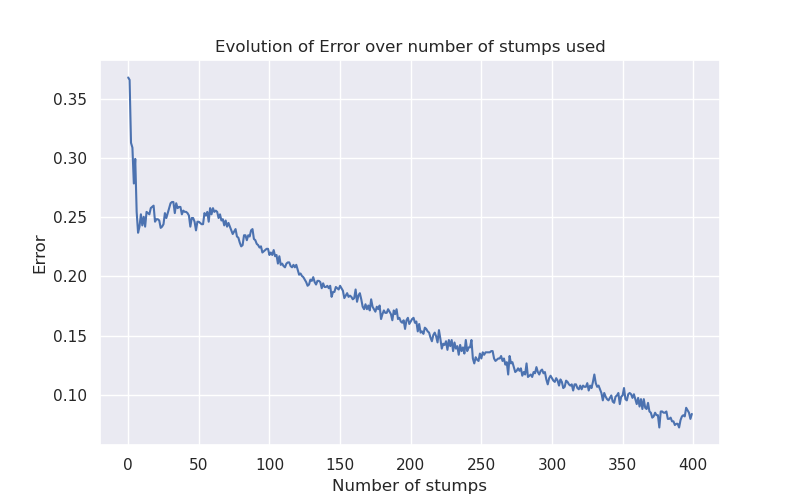
\includegraphics[width=0.8\textwidth]{images/Error.png}
    \caption{Evolução do erro em função do número de estimadores}
\end{figure}

No gráfico acima, como citado, pode ser analisada a variação do erro de
classificação no conjunto de
dados \textit{Tic Tac Toe} conforme aumenta-se o número de estimadores
utilizados. Podemos ver claramente que
com o aumento do número de estimadores, o erro diminui, como era esperado.

Ao aumentar o número de estimadores, o viés no modelo diminui e sua capacidade
de generalização aumenta,
permitindo assim que o erro em dados ainda não vistos seja menor. No entanto,
podemos ver que a partir de certo número
de estimadores (neste caso, aproximadamente 250), o erro do modelo durante a
classificação converge
para um valor específico, e passa a não diminuir mais.

Tal situação pode ser analisada de diversar formas. Primeiramente, é necessário
lembrar que os pesos dos estimadores
diminuem conforme aumenta o número de estimadores utilizados. Ou seja, a partir
de certo ponto, é natural que
novos estimadores causem pouco impacto na classificação, já que seus pesos
serão muito pequenos. O gráfico abaixo
mostra a variação do peso de cada estimador para um modelo classificador da
base \textit{Tic Tac Toe} sem validação cruzada, e permite enxergar esse fato.

\begin{figure}[H]
    \centering
    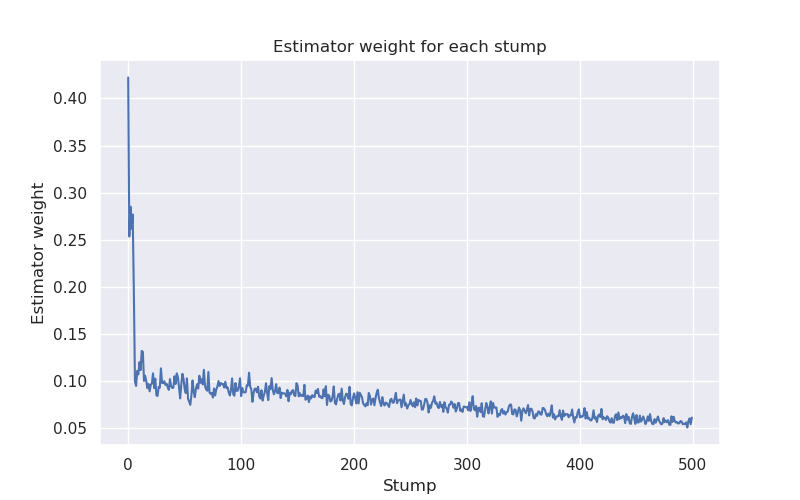
\includegraphics[width=0.8\textwidth]{images/Estimatorweight.png}
    \caption{Evolução do peso de cada estimador}
\end{figure}

Fica evidente que estimadores escolhidos \enquote{mais a frente} terão pesos
menores, e dessa maneira
não causarão tanto impacto no modelo final e, por isso, após certo tempo, o
aumento do número de estimadores
não necessariamente irá tornar o modelo mais poderoso.

Na figura abaixo, pode-se ser vista a evolução da acurácia do modelo conforme o
aumento do número de estimadores
utilizados. Como a acurácia, neste caso, é igual a um menos o valor do erro, a
soma desses dois valores será um e o
gráfico permite enxergar esse fato.

\begin{figure}[H]
    \centering
    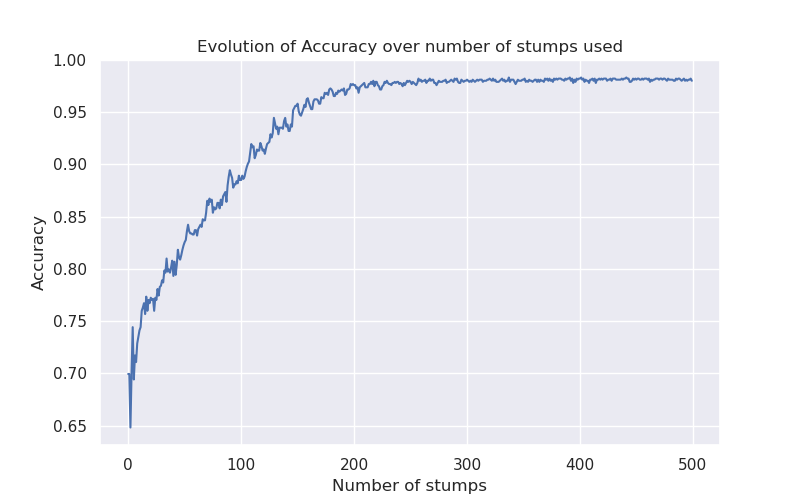
\includegraphics[width=0.8\textwidth]{images/Accuracy.png}
    \caption{Evolução da acurácia em função do número de estimadores}
\end{figure}

Como já foi explicado acima, após certo número de estimadores, a performance do
modelo não
aumenta, uma vez que os pesos desses novos estimadores não irão impactar na
classificação após
certo ponto. Por isso, após aproximadamente 250 estimadores, a acurácia do
modelo parece convergir
para um mesmo valor constante.

\section{Conclusão}

Em suma, após as análises e discussões apresentadas neste relatório, fica
evidente que o
processo de \textit{boosting} é uma metodologia extremamente útil para diminuir
o viés de modelos
extremamente simples. No entanto, conforme visto, o benefício que é trago por
ela possui limites, e seu
uso e implementação deve ser feito de maneira inteligente para tirar o máximo
proveita dela.

\end{document}